\documentclass[10pt,border=4pt]{standalone}
\usepackage{mathptmx}
\usepackage{amsmath,amssymb,bm}
\usepackage{tikz}
\usetikzlibrary{patterns,decorations.pathmorphing,decorations.pathreplacing,arrows.meta,fit,backgrounds,calc,positioning,shapes.geometric}
\definecolor{acc}{HTML}{0B5394}
\definecolor{accl}{HTML}{EAF0F7}
\definecolor{grp}{HTML}{F5F5F5}
\definecolor{org}{HTML}{C55A11}
\definecolor{orgl}{HTML}{FBEFE6}
\tikzset{
 dat/.style={draw=black,line width=0.6pt,fill=white,align=center,font=\small,inner sep=3pt,minimum height=0.85cm},
 lay/.style={draw=acc,line width=0.8pt,fill=accl,rounded corners=2pt,align=center,font=\small,inner sep=3pt,minimum height=0.85cm},
 cnd/.style={draw=org,line width=0.8pt,fill=orgl,rounded corners=2pt,align=center,font=\small,inner sep=3pt,minimum height=0.75cm},
 op/.style={circle,draw=black,line width=0.6pt,fill=white,inner sep=0.5pt,font=\small,minimum size=5mm},
 grpb/.style={draw=black!45,dashed,line width=0.6pt,rounded corners=3pt,inner sep=6pt},
 arr/.style={-{Latex[length=2.2mm,width=1.7mm]},line width=0.7pt},
 carr/.style={-{Latex[length=2.2mm,width=1.7mm]},line width=0.7pt,draw=org},
 shp/.style={font=\scriptsize,text=black!70,inner sep=1pt},
 lab/.style={font=\footnotesize,inner sep=1pt},
 ttl/.style={font=\small\bfseries,inner sep=0pt,anchor=west}
}
\newcommand{\xh}{\mathbf{x}_h}\newcommand{\xf}{\mathbf{x}_f}

\tikzset{vlv/.style={draw=org,line width=0.8pt,fill=orgl,minimum width=1.25cm,minimum height=0.6cm,font=\footnotesize,inner sep=1pt},
 vlh/.style={draw=black!60,line width=0.8pt,fill=grp,minimum width=1.25cm,minimum height=0.6cm,font=\footnotesize,inner sep=1pt},
 cyl/.style={draw=acc,line width=0.8pt,fill=accl,align=center,font=\small,minimum height=1.2cm,minimum width=2.0cm},
 flow/.style={-{Latex[length=2.2mm,width=1.7mm]},line width=1pt,draw=acc}}
\begin{document}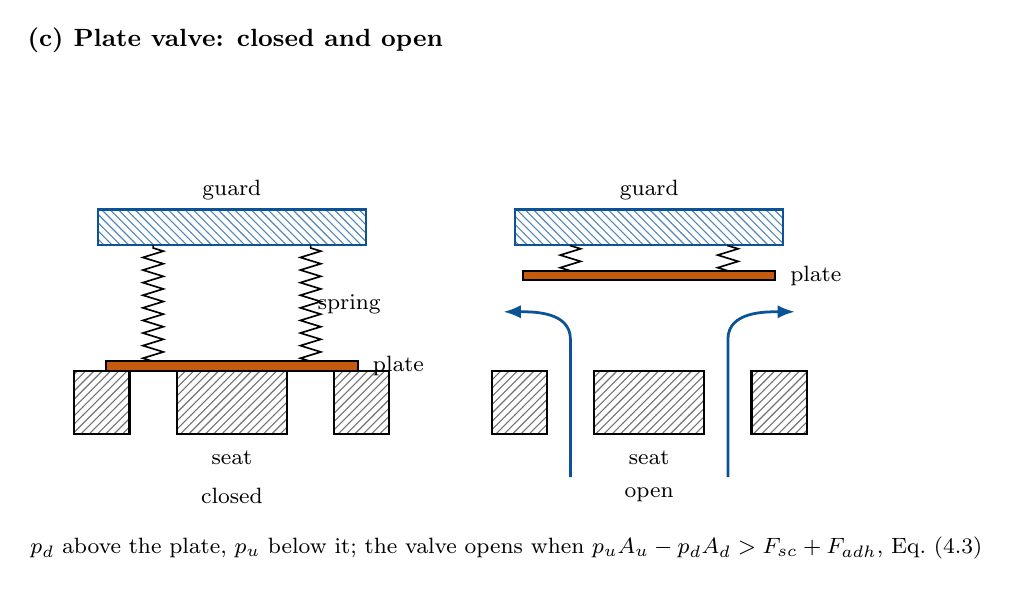
\begin{tikzpicture}[x=1cm,y=1cm]
% ---------------- (c) plate valve
\begin{scope}[shift={(0,0)}]
\node[ttl] at (-0.6,5.0) {(c) Plate valve: closed and open};
\foreach \dx/\op/\tt in {0/0/closed, 5.3/1/open}{
 \begin{scope}[shift={(\dx,0)}]
 % seat with two ports
 \fill[pattern=north east lines,pattern color=black!55] (0,0) rectangle (0.7,0.8) (1.3,0) rectangle (2.7,0.8) (3.3,0) rectangle (4.0,0.8);
 \draw[line width=0.8pt] (0,0) rectangle (0.7,0.8) (1.3,0) rectangle (2.7,0.8) (3.3,0) rectangle (4.0,0.8);
 \node[lab] at (2.0,-0.3) {seat};
 % guard
 \fill[pattern=north west lines,pattern color=acc!70] (0.3,2.4) rectangle (3.7,2.85);
 \draw[line width=0.8pt,draw=acc] (0.3,2.4) rectangle (3.7,2.85); \node[lab] at (2.0,3.1) {guard};
 % plate
 \pgfmathsetmacro{\py}{0.8+\op*1.15}
 \draw[line width=0.8pt,fill=org] (0.4,\py) rectangle (3.6,\py+0.12);
 % springs
 \foreach \sx in {1.0,3.0}{\draw[line width=0.6pt,decorate,decoration={zigzag,segment length=1.6mm,amplitude=1.3mm}] (\sx,\py+0.12)--(\sx,2.4);}
 \node[lab,anchor=west] at (3.75,\py+0.06) {plate}; \ifnum\op=0 \node[lab,anchor=west] at (3.05,{(\py+2.5)/2}) {spring};\fi
 \node[lab,anchor=north] at (2.0,-0.65) {\tt};
 \ifnum\op=1
   \draw[flow,draw=acc] (1.0,-0.55)--(1.0,1.2) to[out=90,in=0] (0.15,1.55); \draw[flow,draw=acc] (3.0,-0.55)--(3.0,1.2) to[out=90,in=180] (3.85,1.55);
 \fi
 \end{scope}}
\node[lab,align=left,anchor=west] at (-0.6,-1.45) {$p_d$ above the plate, $p_u$ below it; the valve opens when $p_uA_u-p_dA_d>F_{sc}+F_{adh}$, Eq.~(4.3)};
\end{scope}
\end{tikzpicture}\end{document}
